\documentclass[12pt,a4paper]{article}
\usepackage[margin=2.5cm]{geometry}
\usepackage{fontspec,polyglossia}
\setmainlanguage[numerals=maghrib]{arabic}
\setotherlanguage{english}
\newfontfamily\arabicfont[Script=Arabic,Scale=1.05]{Amiri}
\usepackage{amsmath,graphicx,algorithm,algpseudocode,hyperref}
\graphicspath{{../../figures/}}
\title{\textbf{WQK-Newton: نيوتن كريلوف التكعيبي المُحمّى شبه-نيوتن}\\
\large \textenglish{L-BFGS} للحوض المحدب و\textenglish{DA-SFCN} للسرج والطور النيوتني}
\author{الورقة 4 من 6 --- مجموعة التحسين العددي}
\date{سبتمبر 2026}
\begin{document}
\maketitle
\begin{abstract}
\textenglish{WQK-Newton} هجين بطورين. الطور الأول $K_0$ خطوات
\textenglish{L-BFGS}، الأسرع عادة في منطقة محدبة معتدلة اللاخطية. والطور
الثاني تحويل إلى \textenglish{DA-SFCN} الذي يوفّر الهروب من الانحناء السالب
وتقاربًا تربيعيًا لا يضمنه \textenglish{L-BFGS}. على اللوجستي غير المحدب يحلّ
الطور الأول المسألة (9 تكرارات، $\|\nabla f\|\approx 2\times 10^{-9}$) فلا
يبدأ الثاني. وعلى روزنبروك يحسّن الهجين قيمة الهدف مقابل \textenglish{L-BFGS}
الصرف ($13.2$ مقابل $18.5$). الخوارزمية تحوّط لا تسوية: كل طور يُشغَّل كما هو.
\end{abstract}

\section{لماذا الهجين؟}
\textenglish{L-BFGS} يبني معكوس هيسيان محدد موجب من أزواج الإزاحة فلا
يستطيع تمثيل انحناء سالب. إنه الأداة الخطأ على سروج \textenglish{Dauphin}
(يفوته هروب واحد من 12؛ \textenglish{DA-SFCN} لا يفوته شيء) والأداة الصحيحة
على أحواض لوجستية. \textenglish{WQK-Newton} ترفض الاختيار.

\section{الخوارزمية}
نشغّل \textenglish{L-BFGS} لـ $K_0$ خطوات أو حتى $\|\nabla f\|\le\varepsilon$.
إن لم يتحقق التقارب نكمل بـ\textenglish{DA-SFCN} من النقطة الحالية.
تحسين مستقبلي طبيعي: حقن أزواج \textenglish{L-BFGS} كمهيئ لـ\textenglish{Lanczos}
في الطور الثاني، وهو ما يوحي به اختبار روزنبروك في الورقة الجامعة.

\section{التجارب}
\begin{figure}[h]
\centering
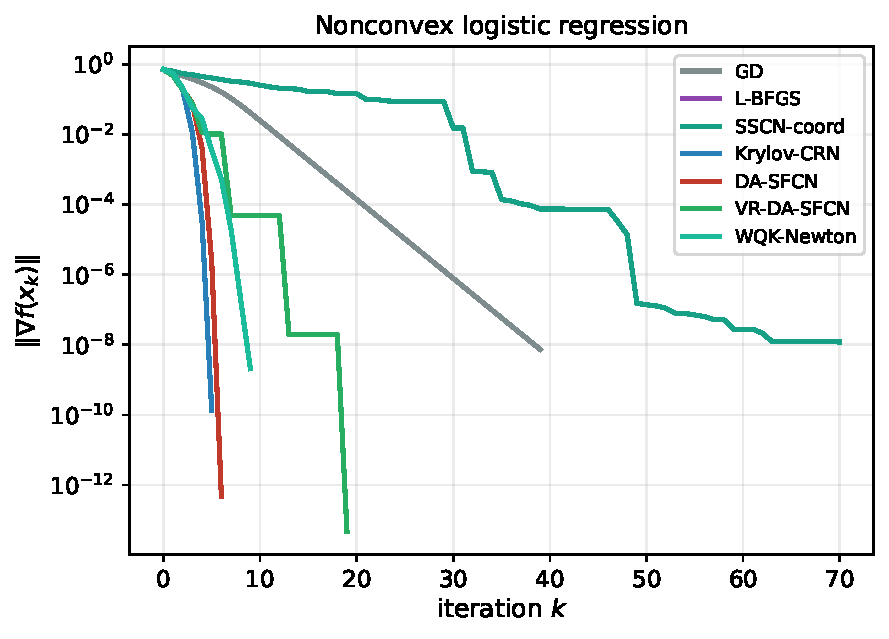
\includegraphics[width=0.48\textwidth]{fig_logistic.pdf}
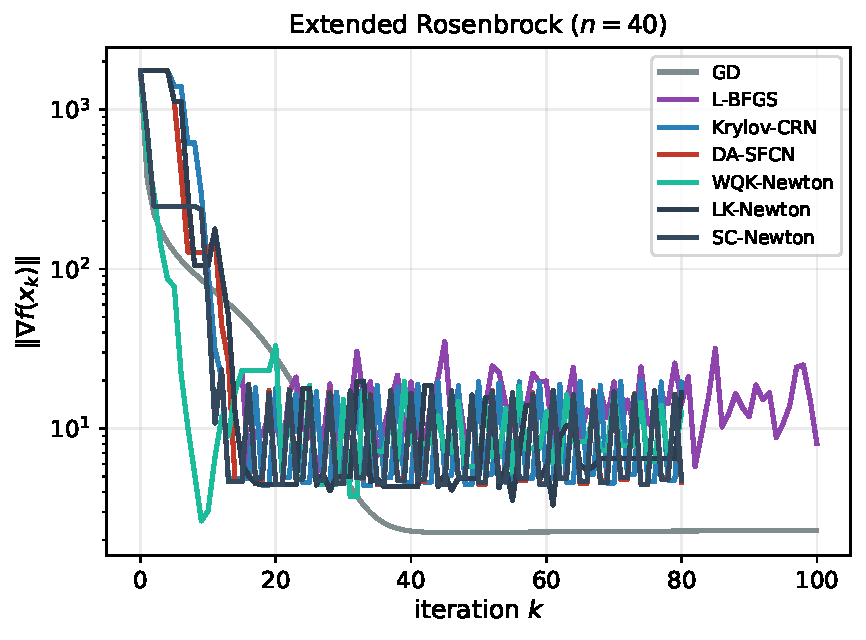
\includegraphics[width=0.48\textwidth]{fig_rosenbrock.pdf}
\caption{اللوجستي غير المحدب (يسار) وروزنبروك الممدَّد (يمين).}
\end{figure}
\begin{figure}[h]
\centering
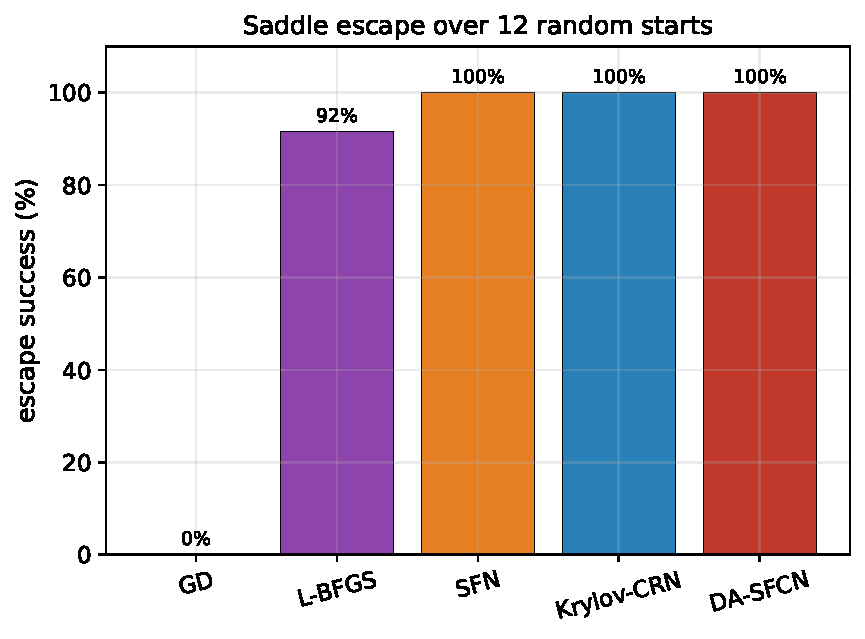
\includegraphics[width=0.48\textwidth]{fig_success.pdf}
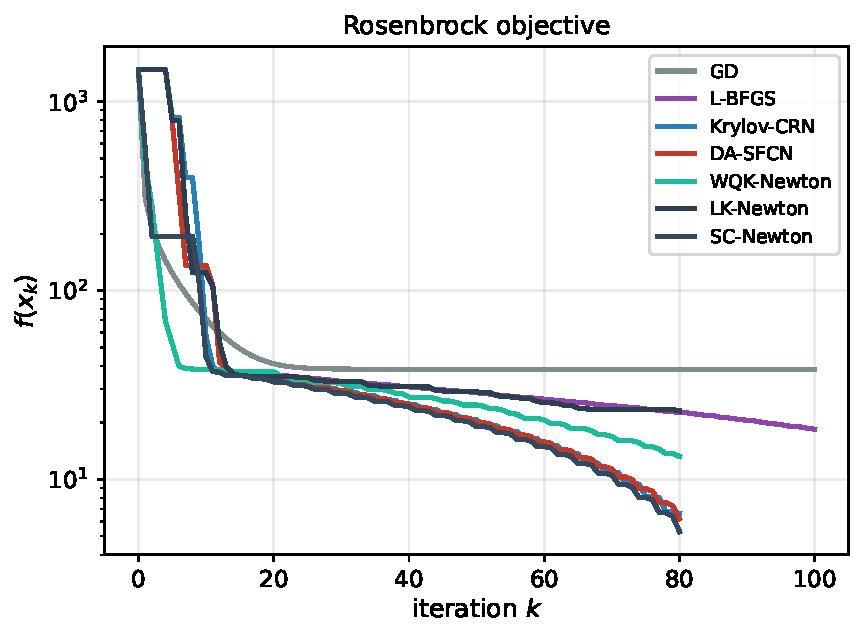
\includegraphics[width=0.48\textwidth]{fig_rosenbrock_f.pdf}
\caption{يسار: \textenglish{L-BFGS} قوي على السروج لكن غير مكتمل. يمين: دالة الهدف.}
\end{figure}

\section{الخاتمة}
\textenglish{WQK-Newton} الافتراضي العملي عندما قد تكون المسألة محدبة
جوهريًا أو غنية بالسروج دون ضبط $m_{\min}$ مسبقًا. تُستخدم معلومات الرتبة
الأولى ثم تُنفق جداءات الهيسيان فقط إن بقيت حاجة إليها.

\begin{english}
\begin{thebibliography}{9}
\bibitem{nocedal2006} Nocedal, Wright. Numerical Optimization, 2006.
\bibitem{dauphin2014} Dauphin et al. \textit{NeurIPS}, 2014.
\bibitem{jiang2024} Jiang et al. \textit{AISTATS}, 2024.
\end{thebibliography}
\end{english}
\end{document}
